Figure~\ref{fig:4:fw} in Chapter~\ref{chap:cc.fw} shows the structure of the
congestion control framework described in this thesis. The framework
categorizes \emph{In-path} sources and \emph{In-band} signaling for
implementing congestion control (corresponds to \emph{Block A} in
Figure~\ref{fig:4:fw}), which are discussed in this chapter. This chapter is
based on our work on congestion control for interactive multimedia
applications, which is documented in \citepub{c:3grc}, \citepub{c:hetrc},
\citepub{c:eval}, \cite{draft.xr.discard.rle},
\cite{draft.xr.bytes.discarded}, \cite{singh:2010.thesis} and
\cite{Singh:control.loops.api}.

In \citepub{c:3grc}, we propose a new congestion control algorithm for the
mobile (e.g., 3G) environment, to be deployed in IP Multimedia System (IMS).
The main distinction between mobile (e.g., 3G, LTE) and other wireless
environments (e.g., 802.11x) is the media streams are transmitted using the
\emph{unacknowledged mode}; the packets corrupted due to bit-errors (e.g.,
wireless interference) are not re-transmitted. Hence, the packets incur low
delay, compared to Wireless LAN where corrupted packets are retransmitted by
the link layer. We evaluate the performance of a sender-driven congestion
control with a receiver-driven congestion control and evaluate the performance
of the proposed congestion control algorithm in a simulated environment (in
ns-2) using real-world 3G traces~\cite{s4.eval.bitrate, 3gppSim}. In
\citepub{c:hetrc}, we extend the approach in \citepub{c:3grc} for deploying on
the Internet and show that the congestion control scheme is deployable. In
\cite{draft.xr.discard.rle} and \cite{draft.xr.bytes.discarded}, we propose
RTCP XR block extensions that indicate the number of bytes discarded and
run-length encoding of discarded packets, respectively. These packets are
discarded by the receiver because they arrived too early or too late to be
played out by the receiver. This information is used as a congestion cue by
the sender.

\cite{Singh:control.loops.api} discusses the application and API requirements
for interactive multimedia congestion control. It describes the two control
loops: a) between the receiver and the sender, and b) between the media
encoder and the sending agent. In the first loop, the receiver notifies the
sender about the current network characteristics. In the second loop, the
sending agent requests a new media bit rate, and the encoder tries at best to
meet it, sometimes under-shooting or over-shooting the requested rate.

Lastly, in \citepub{c:eval} we evaluate the performance of a congestion
control algorithm proposed by Google for WebRTC. We evaluate the performance
in diverse scenarios measuring scalability (\emph{how quickly is the
congestion control able to utilize the available capacity}), self-fairness and
competing against bursty cross-traffic. We evaluate the performance of
web-browsers implementing the congestion control algorithm in our testbed that
emulates the diverse scenarios.

\section{Schemes of Congestion Control}

The congestion control algorithm can be implemented at the sender, at the
receiver, or the sender and receiver operate co-operatively. The
\emph{sender-driven} scheme requires that the receiver measure the current
network condition and signal the observed congestion cues to the sender, which
calculates the sender's estimate and uses it as the new sending rate. In the
\emph{receiver-driven} scheme, the receiver calculates the new sending rate
(receiver's estimate) based on the observed congestion cues, and signals the
new rate to the sender, which on receiving the new rate, adapts the media bit
rate to received value. The \emph{co-operative} scheme is an extension to the
\emph{sender-driven} scheme, in this case, the receiver calculates the
receiver's estimated rate and signals it along with the observed congestion
cues, the sender at its end calculates the sender's estimate based on the
congestion cues and chooses a new sending rate, typically, between the
sender's estimate and the receiver's estimate. Figure~\ref{fig:cc:scheme}
shows the interaction of the sender and receiver for each scheme. The figure
merely shows the media flow in one direction, however, it should be noted that
the media in the simulation and the emulated testbed actually flow in both
directions unless explicitly mentioned. This is mainly done for the
convenience of representation and followed throughout the remainder of the
thesis.

\subsection{Sender-driven Congestion Control Schemes}

\begin{figure}[!t]
  \centerline{
    \subfloat[Sender-driven Scheme]{
      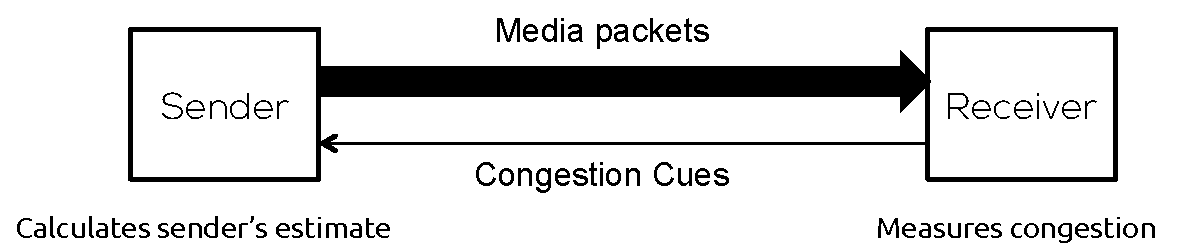
\includegraphics[width=0.9\textwidth]
      {chap5-fig-cc-scheme-s}
    }
  }
  \centerline{
    \subfloat[Receiver-driven Scheme]{
      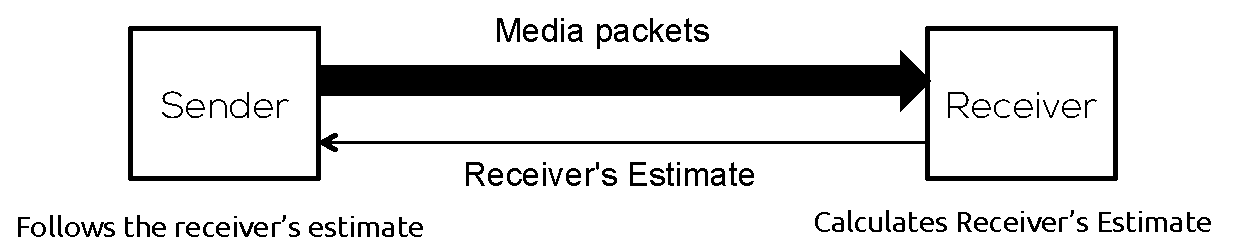
\includegraphics[width=0.9\textwidth]
      {chap5-fig-cc-scheme-r}
    }
  }
  \centerline{
    \subfloat[Co-operative Scheme]{
      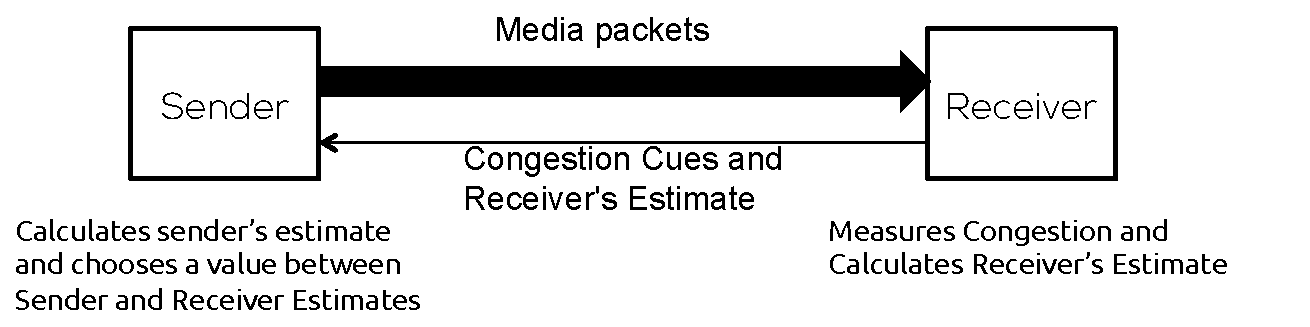
\includegraphics[width=0.9\textwidth]
      {chap5-fig-cc-scheme-c}
    }
  }
  \caption{Congestion control schemes a) sender-driven, b) receiver-driven
and c) co-operative.}
  \label{fig:cc:scheme}
\end{figure}

TCP Friendly Rate Control (TFRC) is an equation based congestion control
algorithm implemented at the sender~\cite{tfrc_347397} and is also implemented
as a profile~\cite{rfc4342} in the Datagram Congestion Control Protocol
(DCCP)~\cite{rfc4340}. TFRC uses the average packet size, round trip time
($RTT$), loss ratio ($p$)~\cite{rfc3448} to calculate the new sending rate.
Formally, the TFRC is calculated as follows:

\begin{align*}
 TFRC = &\; \frac{8 \times avg\_packet\_size}
{RTT \times \sqrt[]{\frac{2 \times b \times p}{3}} + t_{RTP} \times 
\left( 3 \times \sqrt[]{\frac{3 \times b \times p}{8}}\right) \times p \times
\left( 1+32 \times p^2 \right)}\\
where,\; b = &\; 1\\
t_{RTO} = &\; 4 \times RTT
\end{align*}

TFRC cannot be directly be applied to RTP because TFRC requires per-packet
feedback and in RTP, the RTCP feedback is not necessarily sent that
often~\cite{draft.rmcat.feedback}. Therefore, \cite{draft.rtp.tfrc} maps the
TFRC timing rules defined in~\cite{rfc4828, rfc5348} to that of RTP/RTCP
feedback loop, it also proposes extensions to the timing rules in
AVPF-profile~\cite{rfc4585} for very short RTTs ($<20ms$).
\cite{Gharai06:ICME} and \cite{VladBalan:2007dq} show that TFRC is stable on
large RTT paths but less stable for shorter paths, but it also exhibits
saw-tooth behavior~\cite{saurin:2006:thesis}. Any algorithm that consistently
produces a sawtooth media rate is not well suited for real-time communication
because it generates a poor user-experience~\cite{Gharai:2002wt,
Zink03subjectiveimpression}.

Other sender-driven congestion control algorithms are: Rate Adaption Protocol
(RAP)~\cite{rap:752152} uses a windowed-approach and this too exhibits a
sawtooth-type of behavior. Zhu~\textit{et al.}~\cite{rmcat-nada} use
Pre-Congestion Notification (PCN), Explicit Congestion Notification (ECN) and
loss rate to get an accurate estimate delay estimate for implementing
congestion control. In this case, they assume all packets marked by ECN and
PCN as lost. Instead of just relying on RTT and loss for congestion control,
Garudadri~\textit{et al.}~\cite{4397059} also use the receiver playout buffer
to detect underutilization and overuse, i.e., the receiver signals to the
sender the current receiver buffer occupancy. O'Hanlon~\textit{et
al.}~\cite{rmcat-dflow} propose using a delay-based estimate when competing
with similar traffic and using a windowed-approach when competing with
TCP-type cross traffic, they switch modes by using a threshold on the observed
end-to-end delay, the idea is similar to the one discussed
in~\cite{budzisz2011fair}.




\subsection{Receiver-driven Congestion Control Schemes}

In receiver-driven congestion control, the receiver estimates the rate
notifies the sender about the new sending rate. Temporary Maximum Media
Bit-rate Request (TMMBR) is defined as a codec control messages in
\cite{rfc5104}, it is generated by the receiver in a point-to-point video
call. The receiver calculates the new estimate (available capacity) based on
the average inter-arrival time of RTP packets (\emph{video frames}). When the
inter-arrival time of the video frames increases beyond the expected arrival
time in an observed period, the receiver senses \emph{over-use}. When the
frames arrive early, the receiver senses \emph{under-use}. If the over-use and
under-use occur at short timescales, mainly because of I-frames, the receiver
ignores the congestion event. The I-frames are large frames because they are
spatially compressed and are not temporally correlated to previous frames.
Hence, these I-frames are expected to observe queuing delay. The receiver
based on the \emph{over-use} and \emph{under-use} events modifies the
\emph{receiver's capacity estimate}. The receiver sends the TMMBR message to
the sender indicating the maximum sending rate. Currently, interactive
multimedia session in 3GPP~\cite{3gpp.26.114} use TMMBR messages to notify the
sender of the expected sending rate. In WebRTC~\cite{jennings:2013:webrtc},
TMMBR is expected to be used initially, before RTP congestion control is
standardized by the IETF~\cite{rtp-usage}. The expectation is that different
WebRTC clients may develop proprietary receiver-driven algorithms and use
TMMBR as the standardized mechanism to communicate the capacity estimate to
the sender, which will blindly follow it.


\subsection{Co-operative Congestion Control Schemes}
\label{cc:co-op}

Next Application Data Unit (NADU) signaling for video
streaming~\cite{nadu.1070341,nadu.1530486}. NADU is designed for rate
adaptation for video streaming in 3GPP~\cite{3gpp.26.234}. A NADU receiver
measures the playout delay (as a measure of buffer occupancy in time) and
signals it to the sender along with the next sequence number to be played out.
Conversational NADU (C-NADU) is an extension to NADU for congestion control
for interactive multimedia and is described in \citepub{c:3grc} and
\citepub{c:hetrc}. In C-NADU, the receiver also calculates the
\emph{receiver's capacity estimate} by measuring the frame inter-arrival time
and signals that along with the NADU report. If the video frame arrives at the
expected time, the receiver estimates no ongoing congestion, and if it arrives
later than the expected time, it is considered late and the receiver estimates
overuse. If the frame is delayed and misses its playout time, it is discarded
and in this case the receiver estimates congestion. Based on the above cases,
the receiver estimates the current capacity and signals it to the sender. At
the sender, the C-NADU controller, calculates the TCP-friendly rate, measures
the variation in RTT ($75$ and $90$ percentile values), calculates the
fraction of video frames that missed their playout deadline. Based on these
congestion cues and the receiver estimate, the sender chooses a new sending
rate.


Receiver-side Real-Time Congestion Control (RRTCC) is described in
\cite{draft.rrtcc} and is proposed as one of the solution candidates for
WebRTC by Google. Like C-NADU, RRTCC also has a receiver- and sender-side
component. The receiver-side measures the capacity overuse and underuse by
monitoring the timestamp jitter of the incoming frames. The arrival-times are
modeled as a white Gaussian process; when the mean is 0 there is no
congestion, the mean is expected to increase when there is ongoing congestion
and expected to decrease when the congestion abates. Based on this
expectation, the receiver calculates the capacity estimate and signals it to
the sender. The sender calculates its estimate based on TFRC and finally,
chooses the new sending rate as a value between the TFRC rate calculated by
the sender and receiver estimate. Full details of the algorithm proposed by
Google are documented in an Internet-Draft~\cite{draft.rrtcc}.



\begin{figure}[!t]
  \centerline{
    \subfloat[TFRC]{
      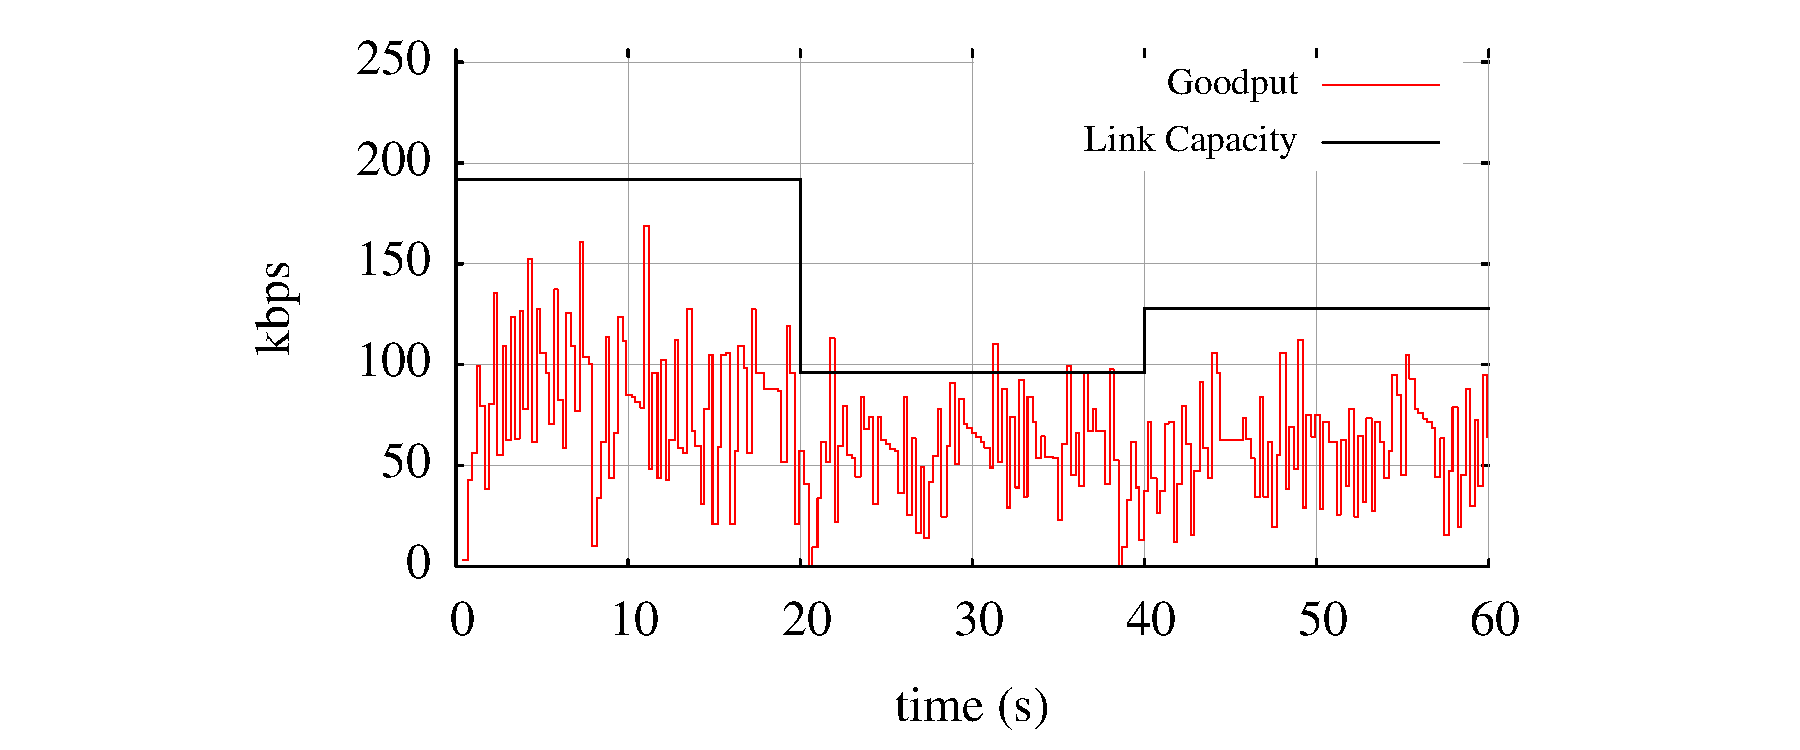
\includegraphics[width=0.5\textwidth, clip=true, trim=3cm 0 4.5cm 0]
      {chap5_graph_sl_tfrc}
    }
    \subfloat[TFRC]{
      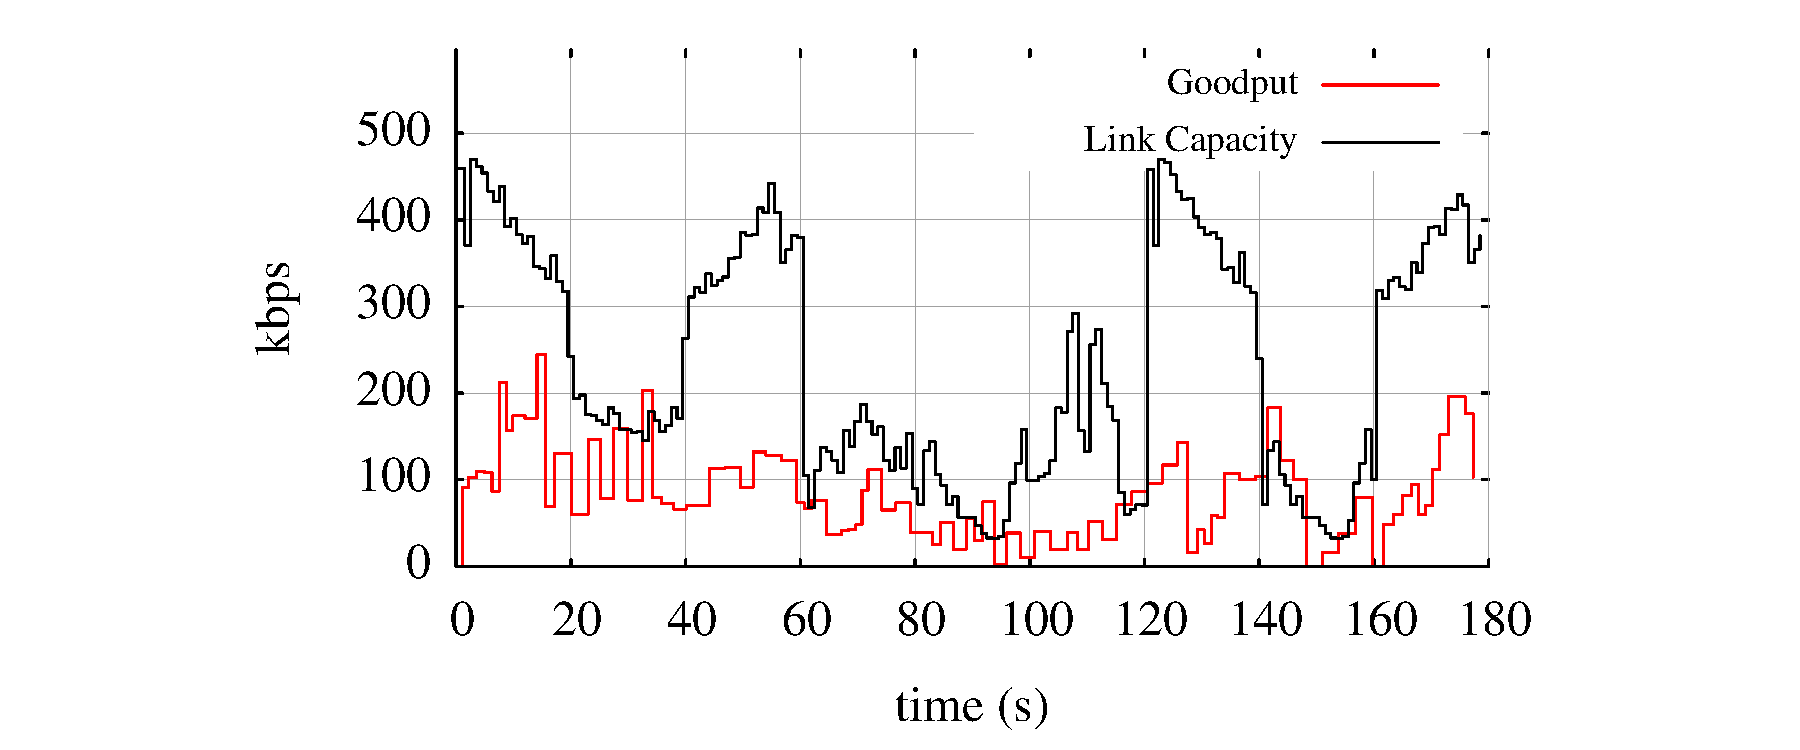
\includegraphics[width=0.5\textwidth, clip=true, trim=3cm 0 4.5cm 0]
      {chap5_graph_3g_tfrc_1}
    }
  }
  \centerline{
    \subfloat[TMMBR]{
      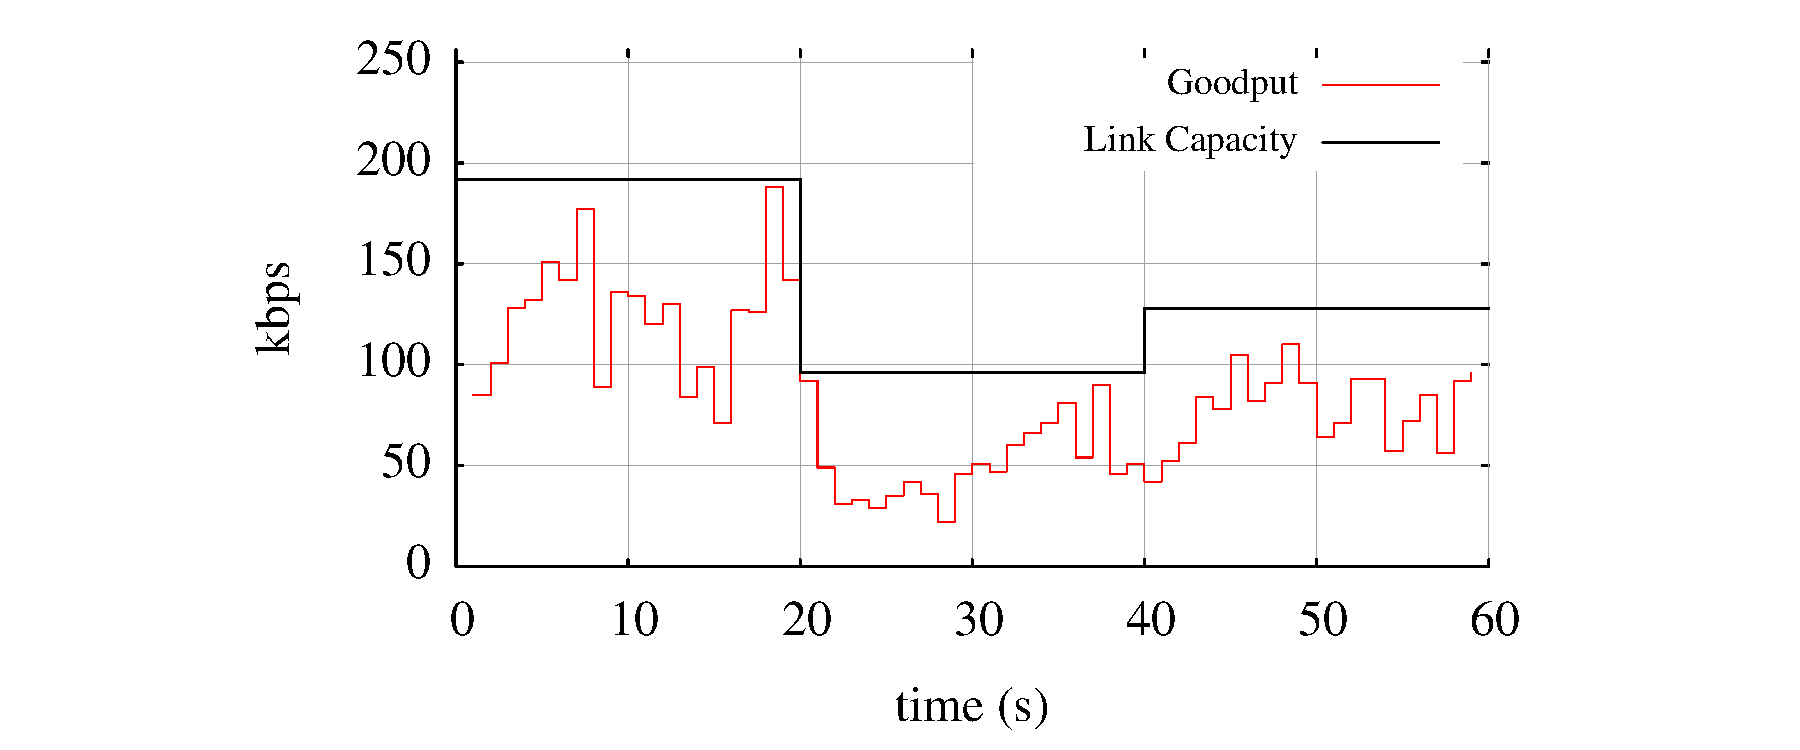
\includegraphics[width=0.5\textwidth, clip=true, trim=3cm 0 4.5cm 0]
      {chap5_graph_sl_tmmbr}
    }
    \subfloat[TMMBR]{
      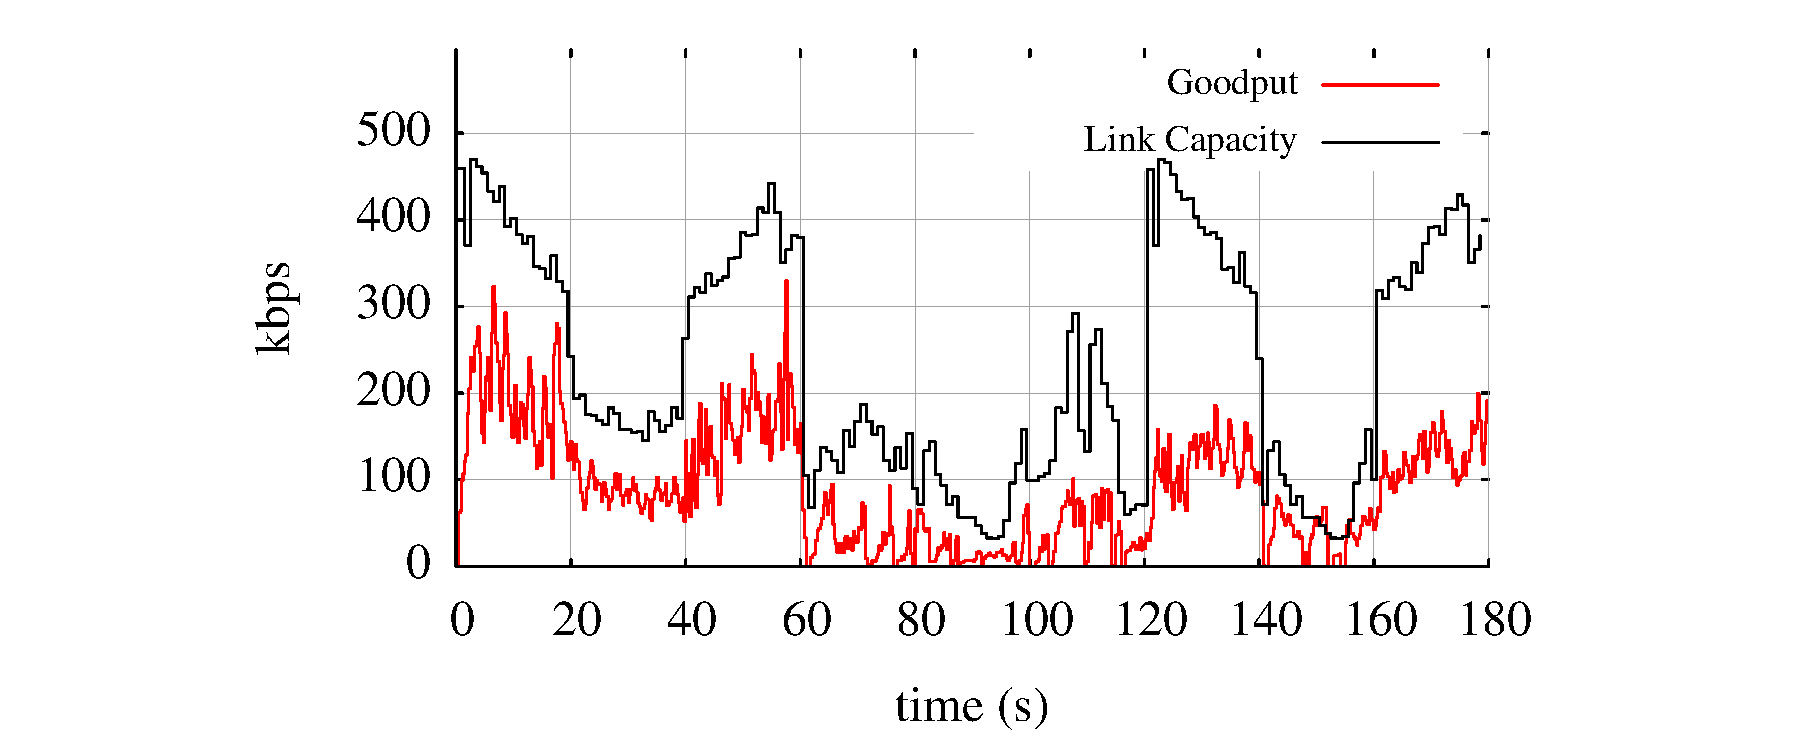
\includegraphics[width=0.5\textwidth, clip=true, trim=3cm 0 4.5cm 0]
      {chap5_graph_3g_tmmbr_u}
    }
  }
  \centerline{
    \subfloat[C-NADU]{
      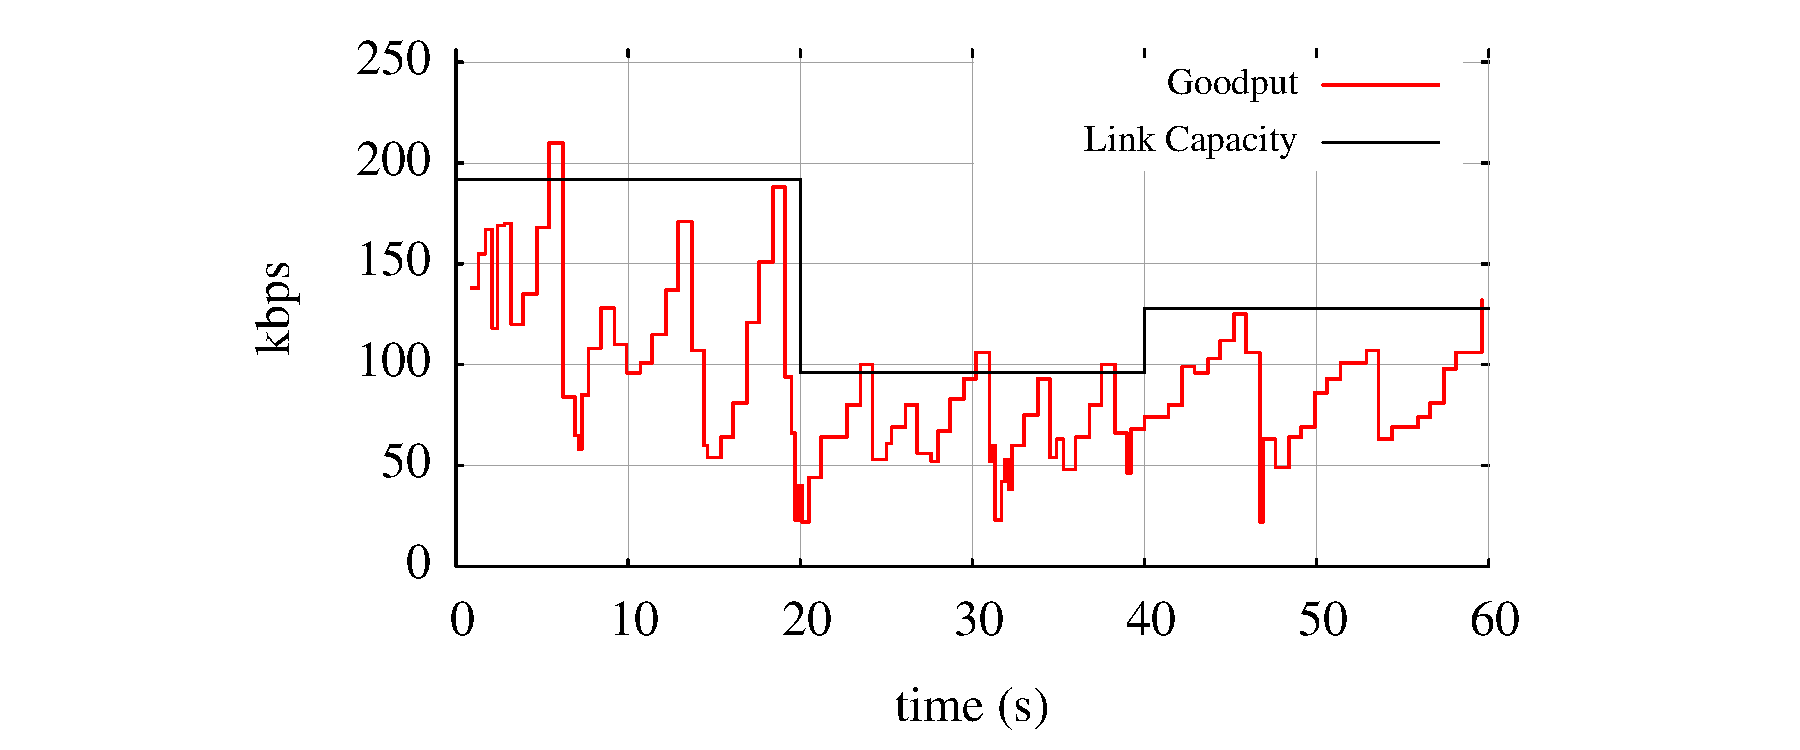
\includegraphics[width=0.5\textwidth, clip=true, trim=3cm 0 4.5cm 0]
      {chap5_graph_sl_cnadu}
    }
    \subfloat[C-NADU]{
      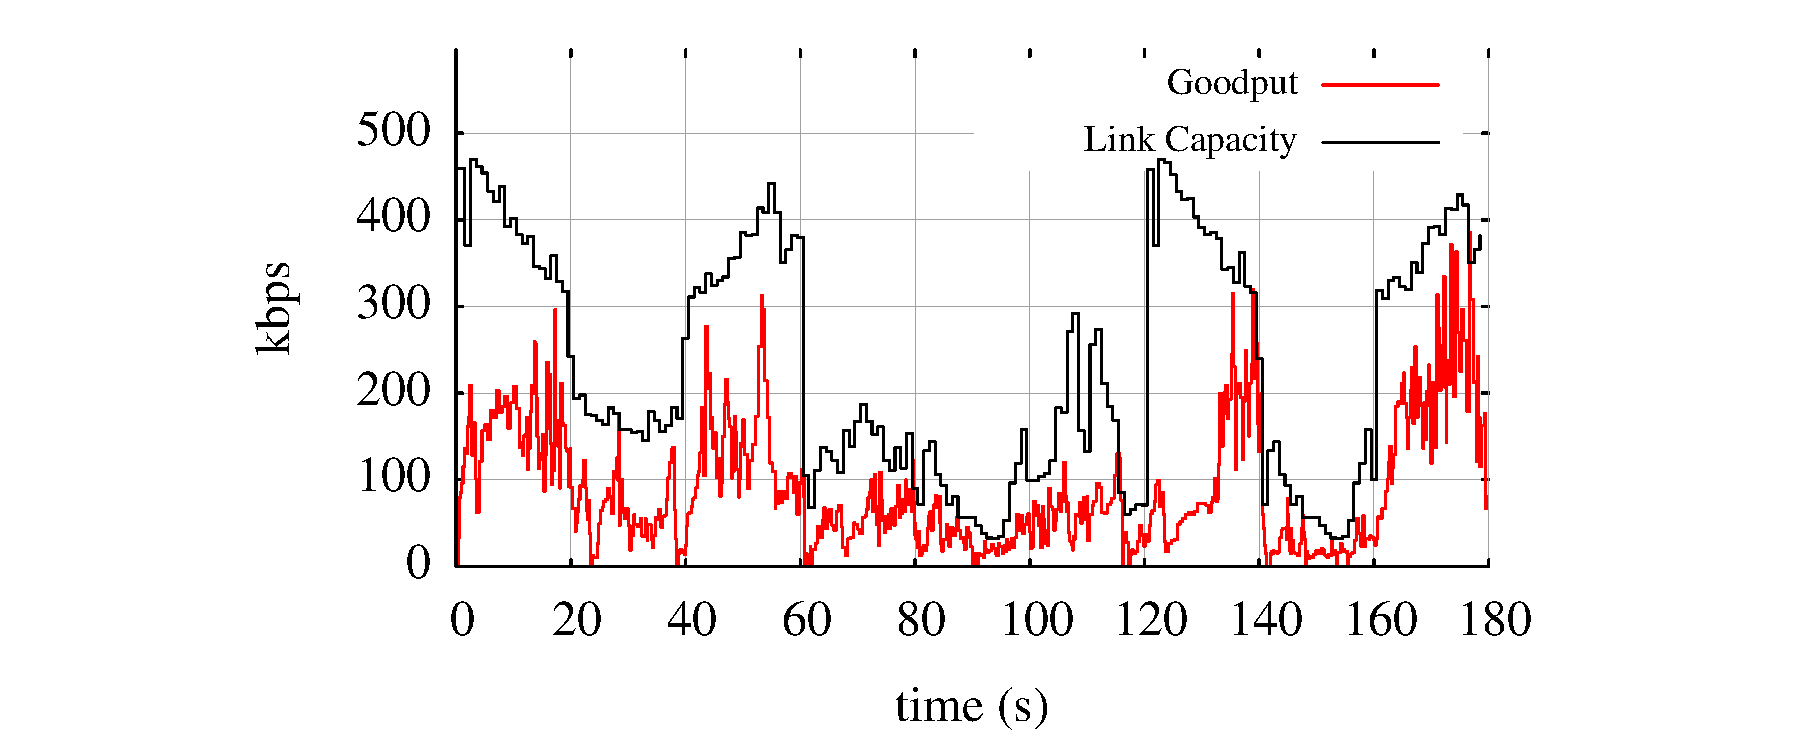
\includegraphics[width=0.5\textwidth, clip=true, trim=3cm 0 4.5cm 0]
      {chap5_graph_3g_cnadu}
    }
  }
  \caption{Performance of TFRC, TMMBR and C-NADU in a slow time-varying (a, c,
  e) link and 3G network (b, d, f).}
  \label{fig:3grc}
\end{figure}


\begin{table}[!t]
\centering{
\begin{tabular}{cccc}
\hline
 & Avg. goodput & PLR & Avg. PSNR\\
 & (kbps)  &(\%) & (dB)\\
\hline
TFRC & 84.1 & 6.9\%& 29.3 \\ %
TMMBR & 89.8 & 3.7\% & 30.5 \\ %
%NADU & 106 & 93 & 29.9& 6.3\%\\%
C-NADU & 92 & 2.2\% & 31.9 \\%
\hline
\end{tabular}
}
\caption{Comparing TFRC, TMMBR, C-NADU for calls over mobile nodes (180s
simulations using 3G traces).}
\label{table:3grc}
\end{table}

\section{Performance Analysis of TFRC, TMMBR, C-NADU, RRTCC}

Our results in \citepub{c:3grc} shows that TFRC produces a sawtooth sending
rate, similar to the performance in~\cite{saurin:2006:thesis}. When the media
stream is the only flow on the end-to-end path, we also observe the average
bandwidth utilization (ABU) is between 30-40\%, i.e., TFRC underutilizes the
link and the loss ratio is about 6\% which results in a lower PSNR compared to
the other two schemes (see Table~\ref{table:3grc}). TMMBR-based congestion
control utilizes the link better than TFRC (ABU between 50-70\%) and produces
a lower loss ratio ($\approx$3\%). Lastly, C-NADU has comparable bandwidth
utilization (ABU=55-60\%) and loss ratio ($\approx$2\%) to TMMBR.
Figure~\ref{fig:3grc} shows the performance of TFRC, TMMBR and C-NADU over two
types of bottleneck links, a slow time-varying link and a 3G link.


\begin{figure}[!t]
\centerline{
%\hfill
\subfloat [Call 1 vs Call 2] {\label{fig_sim-mixed-1-1}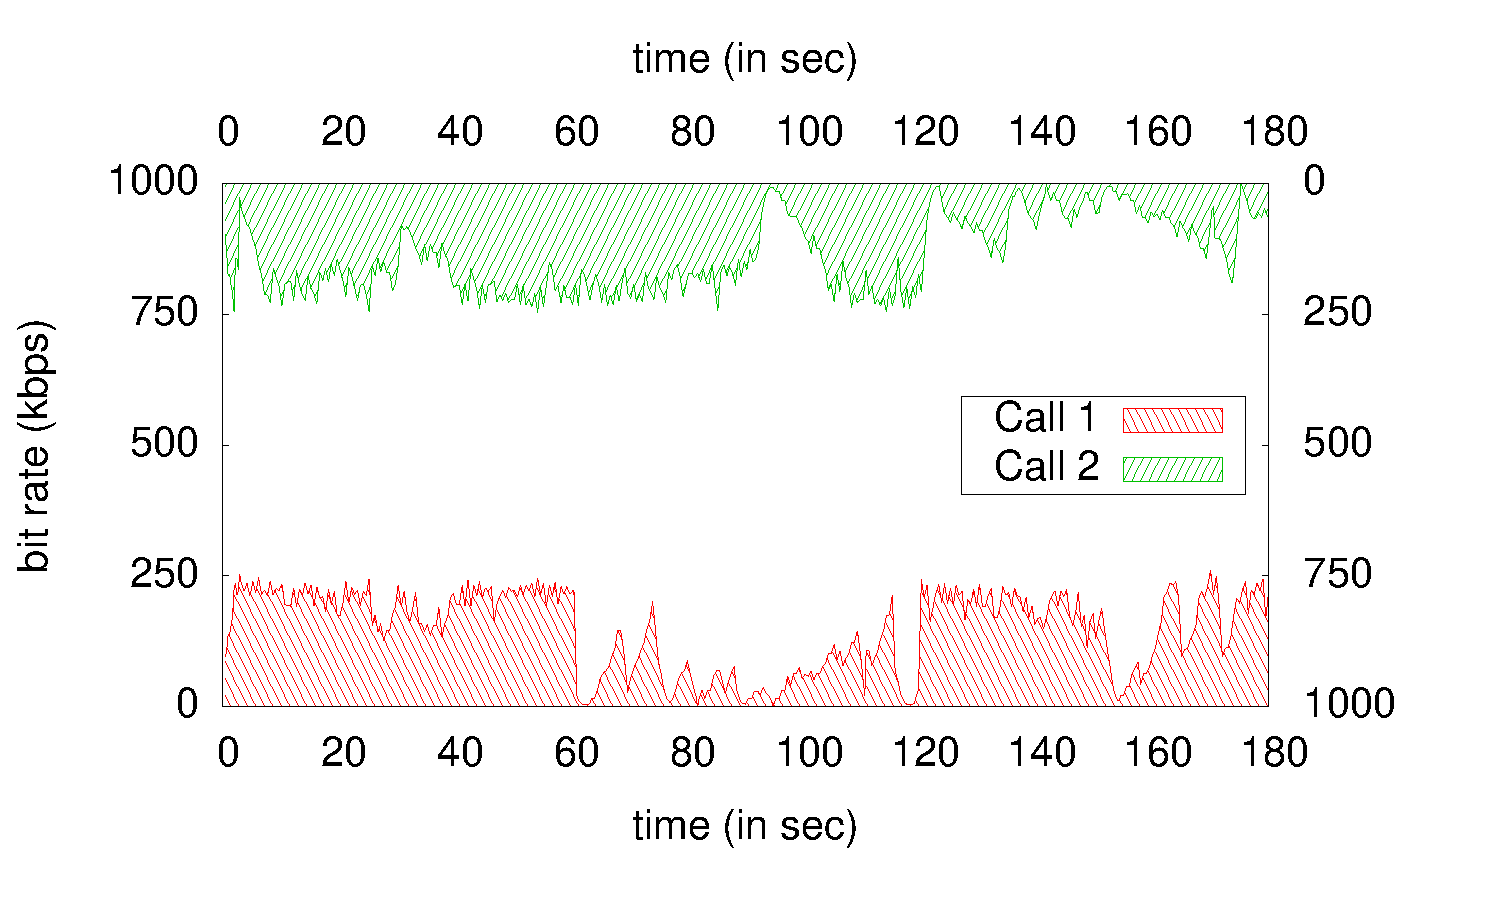
\includegraphics[width=0.5\textwidth]{chap5_5rtp_uc1_12}%
}
%\hfill
\subfloat [Call 1 vs Call 3] {\label{fig_sim-mixed-1-2}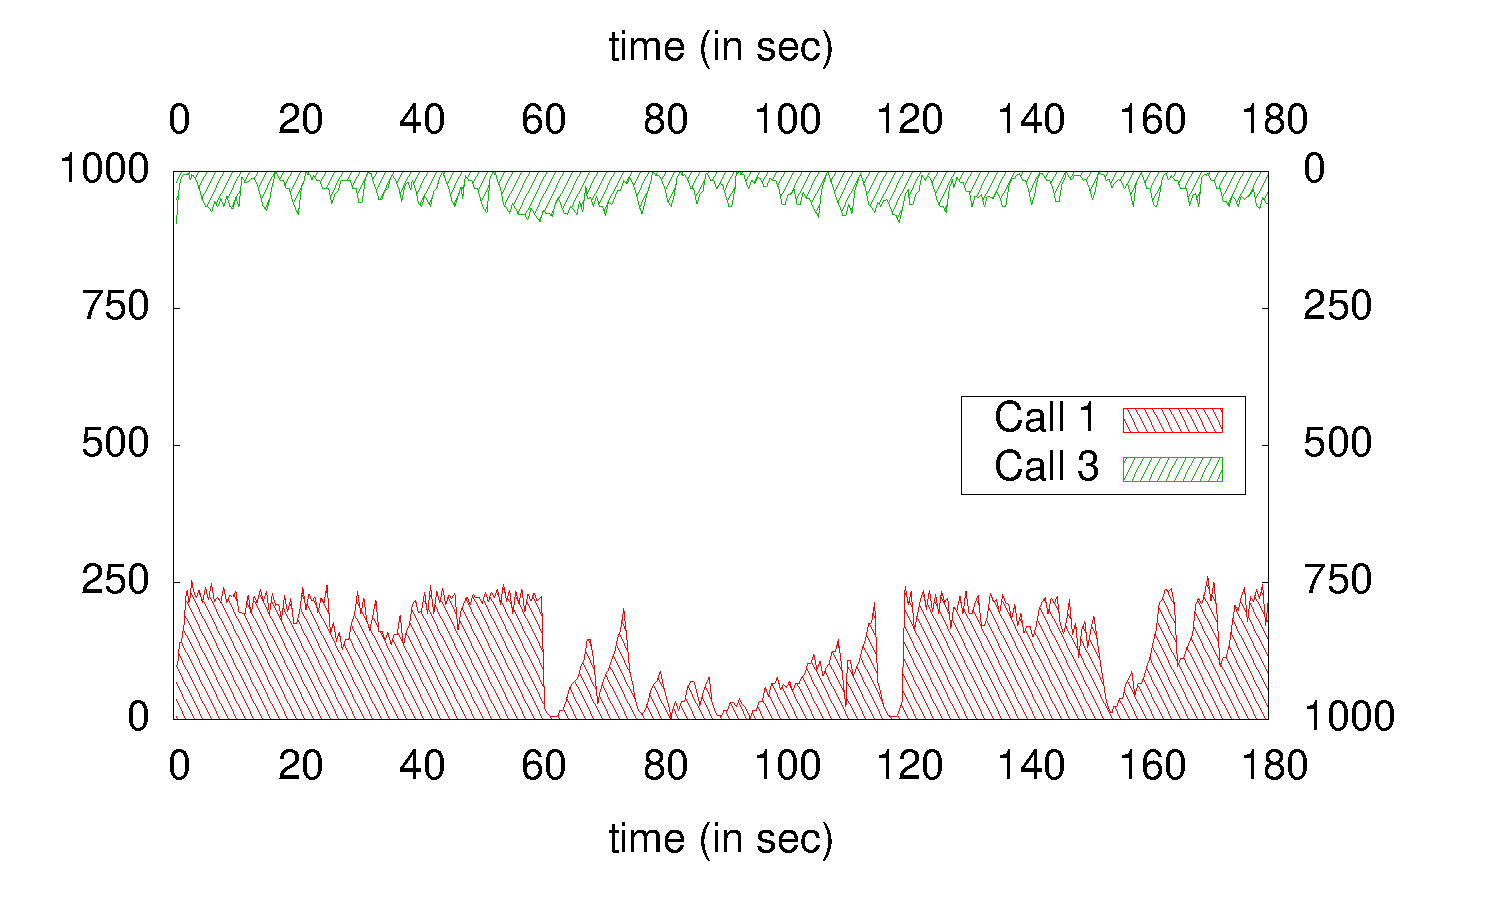
\includegraphics[width=0.5\textwidth]{chap5_5rtp_uc1_13}%
}
%\hfill
}
\centerline{
%\hfill
\subfloat [Call 1 vs Call 4] {\label{fig_sim-mixed-1-3}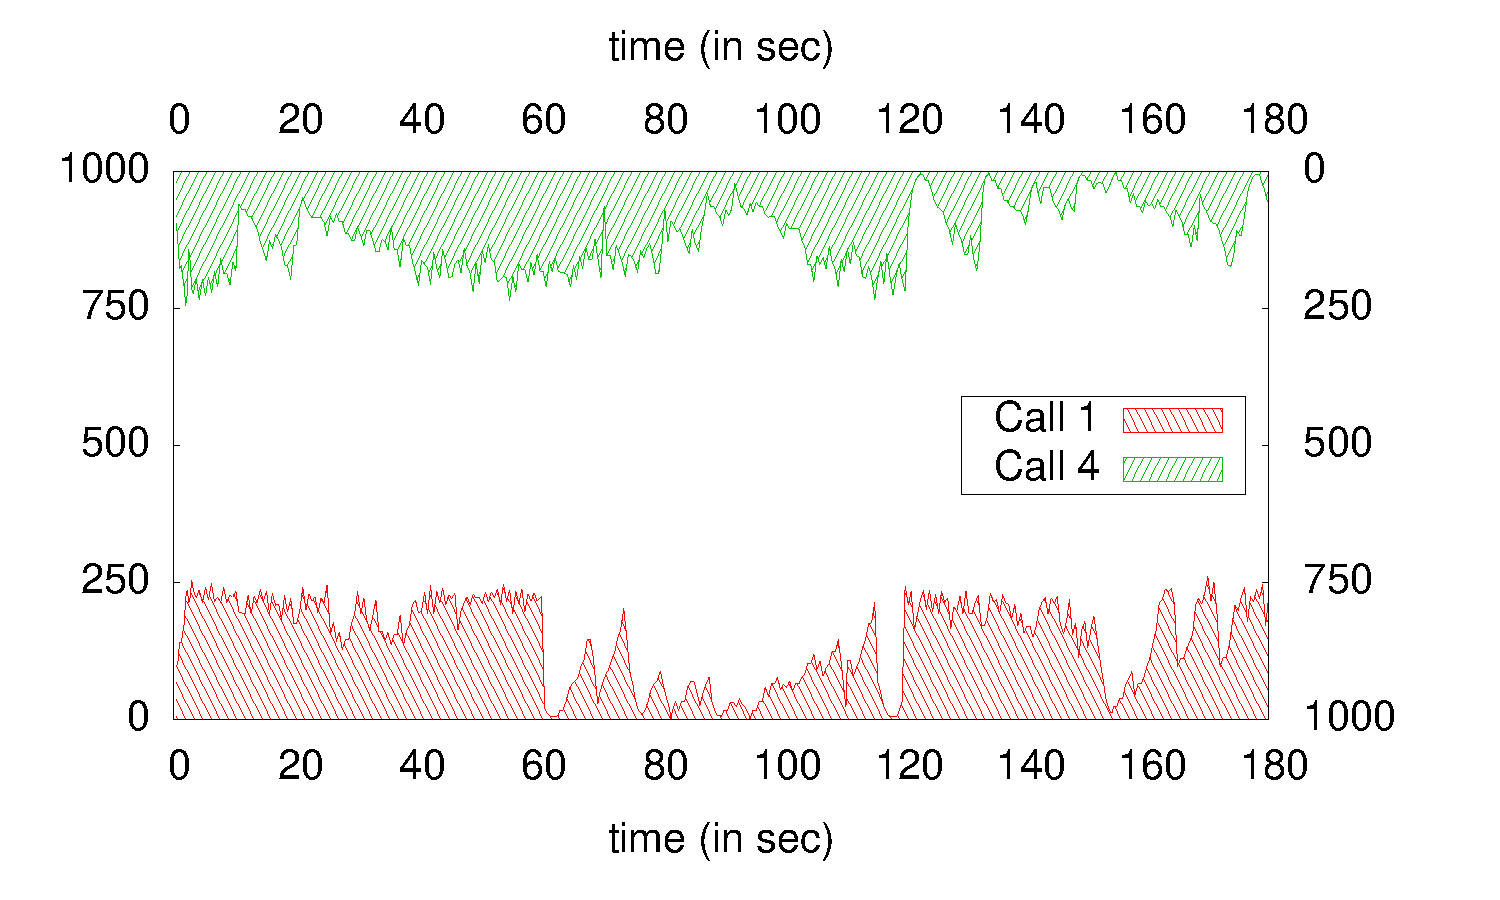
\includegraphics[width=0.5\textwidth]{chap5_5rtp_uc1_14}%
}
%\hfill
\subfloat [Call 1 vs Call 5] {\label{fig_sim-mixed-1-4}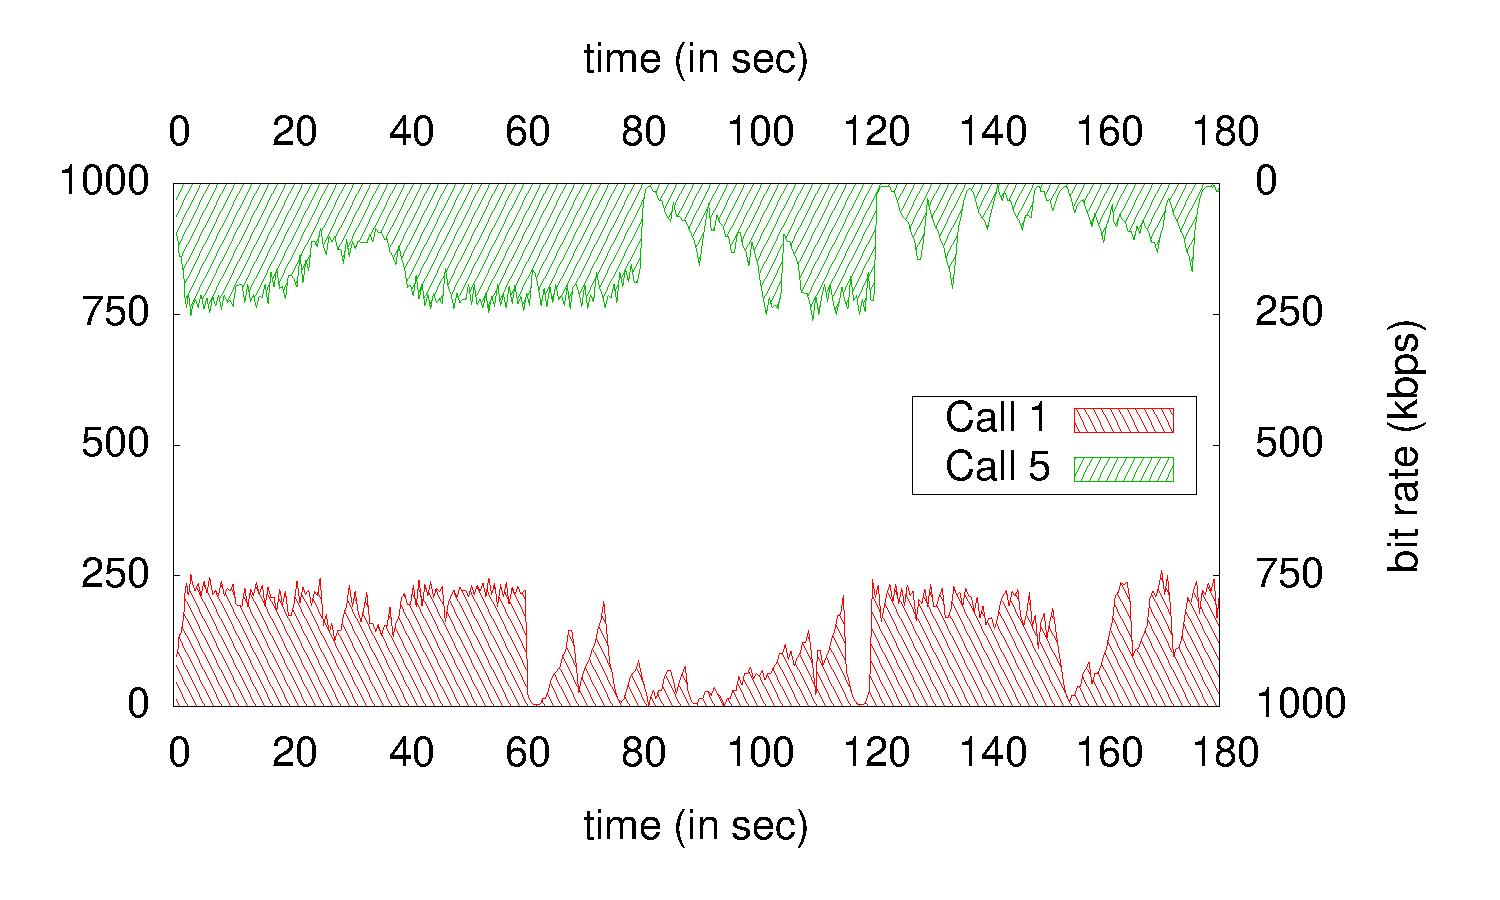
\includegraphics[width=0.5\textwidth]{chap5_5rtp_uc1_15}%
}
%\hfill
}
\caption{C-NADU: Goodput of five calls competing for capacity on a shared
bottleneck in a heterogeneous network. Each calls needs to quickly adapt to
changes in 3G link capacity and fairly share the bottleneck link.}
\label{fig:hetrc}
\end{figure}

\begin{table}[!t]
\centering{
\scalebox{0.9}{
\begin{tabular}{cccccc}
\hline
 & 3G Capacity & $Goodput_{avg}$ & PLR & $PSNR_{avg}$ & ABU \\
 & Pattern & (kbps) & (\%) & (dB) & (\%) \\ 
\hline
Call 1 & Excellent-Poor-Elevator & 140.10 & 2.15\% & 31.4 ($\sigma=0.39$) & 70.1\% \\ 
Call 2 & Good-Good-Poor & 133.55 & 1.61\% & 31.9 ($\sigma=0.62$)& 66.8\% \\ 
Call 3 & Poor-Poor-Poor & 35.18 & 1.55\% & 22.2 ($\sigma=1.13$)& 17.59\% \\ 
Call 4 & Fair-Fair-Poor & 114.96 & 2.75\% & 31.1 ($\sigma=0.75$)& 57.5\% \\ 
Call 5 & Excellent-Elevator-Poor & 130.23 & 2.25\% & 31.3 ($\sigma=0.13$)& 65.1\% \\ 
\hline
\end{tabular}
}}
\caption{C-NADU: Five calls in a heterogeneous network with end-to-end latency
between \emph{60-120ms} and 0.5\% link-layer losses.}
\label{table:hetrc}
\end{table}

In \citepub{c:hetrc}, we show that C-NADU is self-fair with other C-NADU flows
in both wired and wireless environments~\cite{singh:2010.thesis} and in
\citepub{c:fecrc} we show that it competes fairly with TCP cross-traffic, both
long and short (bursty) TCP flows. Figure~\ref{fig:hetrc} show 5 video calls,
each sender uses an independent 3G link into a common bottleneck to the
receivers. The 3G links are based on radio link traces and have different
capacities. Hence, at some instances of time the 3G link is the constraint and
at other times the shared bottleneck link. Table~\ref{table:hetrc} shows that
4 calls have comparable performance (see PSNR and goodput) and 1 call suffers
due to poor connectivity (the 3G link has insufficient capacity which affects
the quality).

\begin{figure}[!t]
  \centerline{
    \subfloat{
      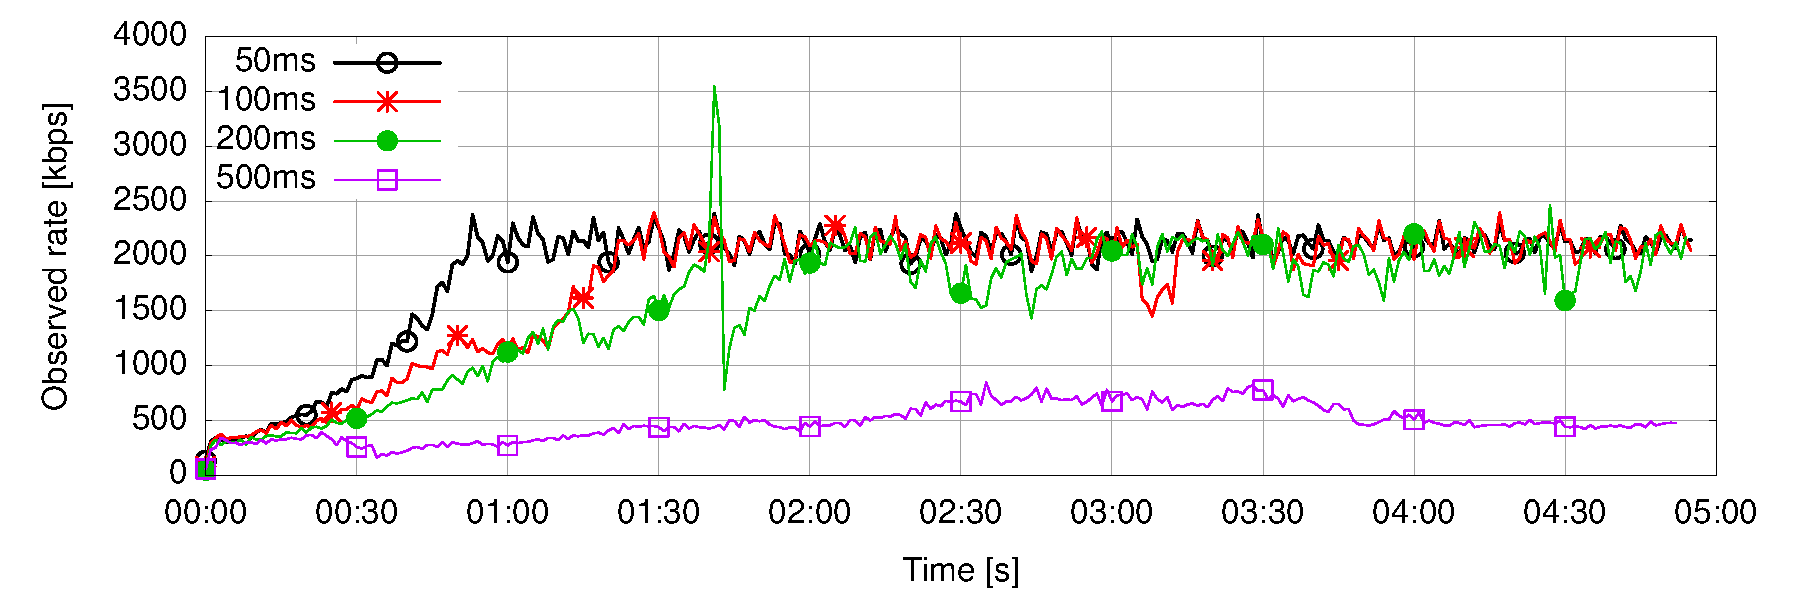
\includegraphics[width=0.8\textwidth]
      {chap5-graph-rrtcc-latency}
    }
   }
   \centerline{
    \subfloat{
      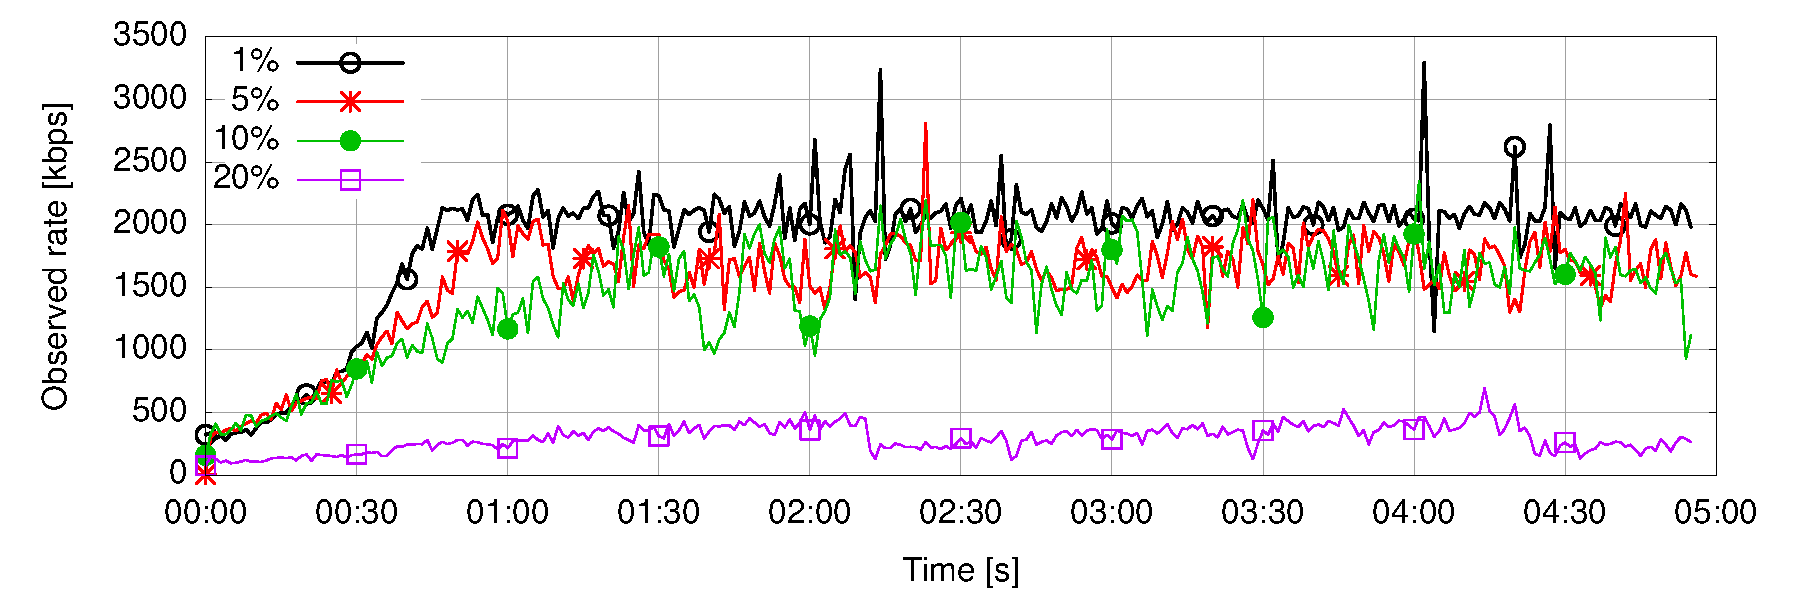
\includegraphics[width=0.8\textwidth]
      {chap5-graph-rrtcc-plr}
    }
  }
  \caption{Performance of RRTCC on a link with varying delay and fractional
  loss rate. We observe that by the sending rate decreases when increasing
  link latency or bit-error loss. }
  \label{fig:rrtcc-single}
\end{figure}

\begin{table}[!t]
\begin{center}{
\begin{tabular}{ ccccc }
\hline
 & Goodput & Residual  & PLR\\
 & (Kbps)  & Loss (\%) & (\%)\\
\hline
 0\% & 1949.7$\pm233.62$ & 0.011 & 0.011 \\ 
 5\% & 1568.74$\pm178.52$ & 0.23 & 9.77 \\ 
 10\% & 1140.82$\pm161.92$ & 0.49 & 19.02 \\ 
 20\% & 314.4$\pm61.98$ & 2.43 & 36.01 \\ \hline
\end{tabular}
}
\end{center}
\caption{RRTCC: Metrics for a bottleneck with different packet loss rates.}
\label{tab:rrtcc-loss}
\end{table}

In \citepub{c:eval}, we evaluate the performance of RRTCC in several
scenarios: by itself on a bottleneck link, competing with other RRTCC flows
and competing with TCP cross-traffic. Figure~\ref{fig:rrtcc-single} shows an
example plot of the performance of RRTCC when increasing latency and
fractional loss. For example, in Figure~\ref{fig:rrtcc-single}(a) by
increasing the bottleneck link latency reduces the sending rate of RRTCC.
Similarly, Figure~\ref{fig:rrtcc-single}(a) shows that increasing the loss
rate also affects the sending rate. However, we observe that even though the
link has high loss rate, the residual loss rate is low (even when the loss is
20\%), mainly due to the use of NACKs, PLI and FEC.


\begin{figure}[!t]
\centerline{
  \subfloat[Start together]
    {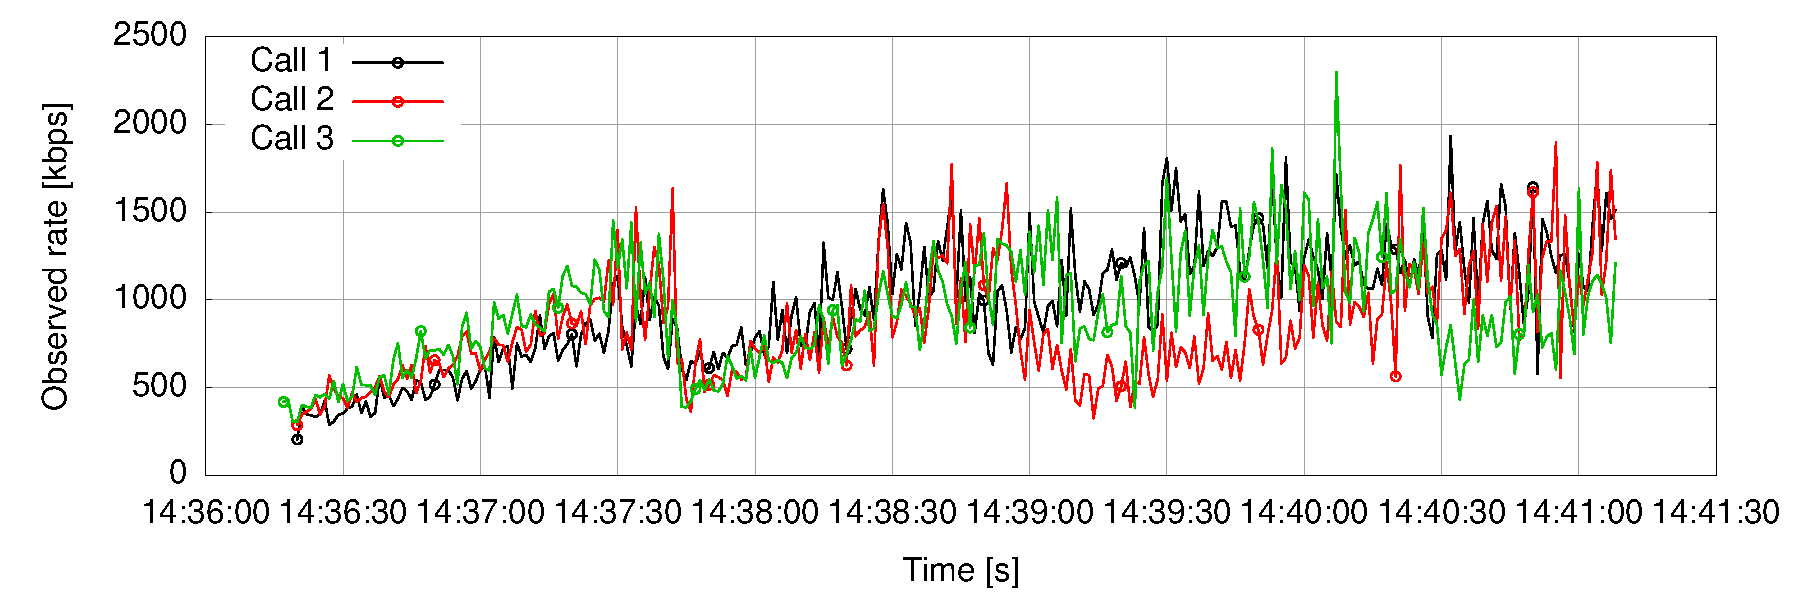
\includegraphics[width=0.8\textwidth]{chap5_sync_three-calls}}
  }
  \centerline{
  \subfloat[Start 30s apart]
    {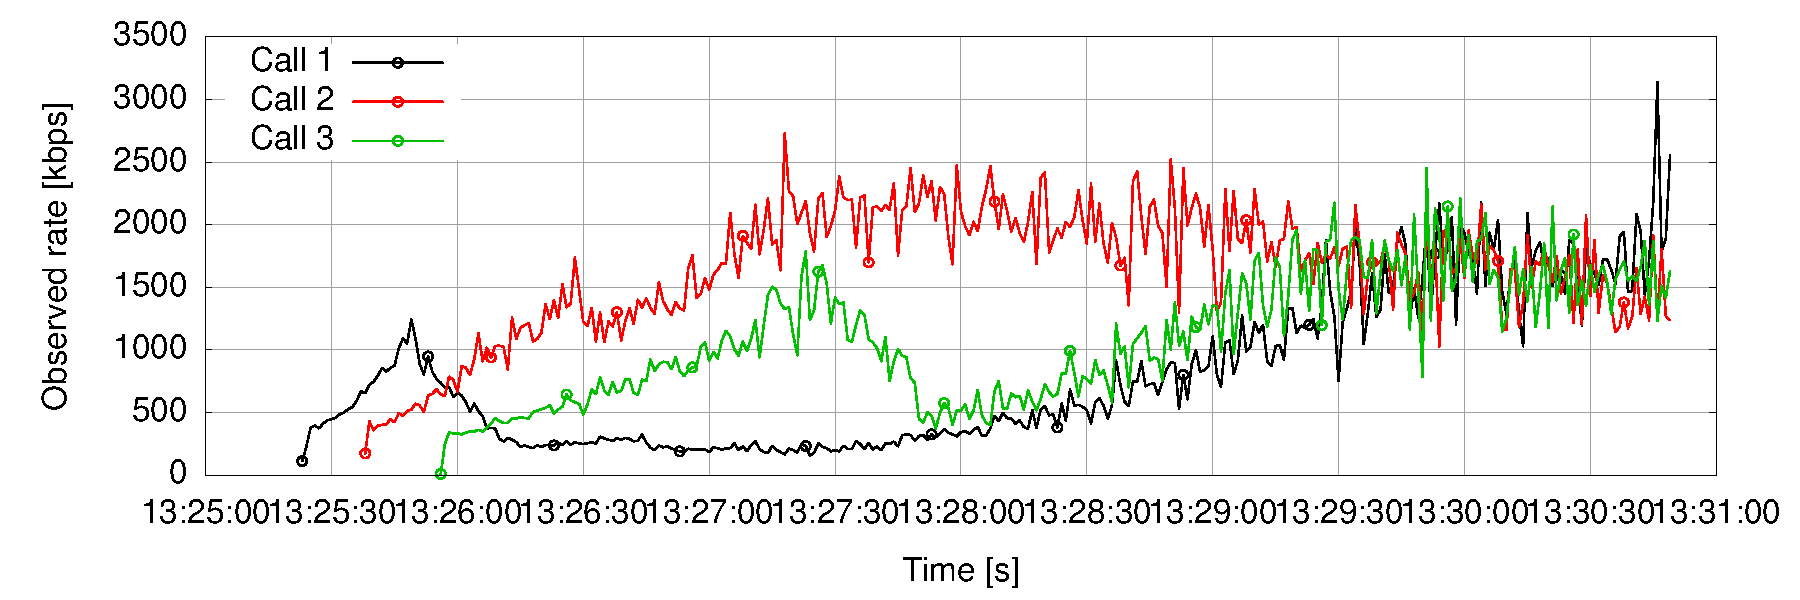
\includegraphics[width=0.8\textwidth]{chap5_async3_three-calls}}
  }
   \caption{RRTCC: Variation in receiver rate for 3 parallel calls a) starting
   together, b) starting 30s apart. The total duration of the call is 5 mins
   (300s).}
\label{fig:rrtcc-self-fair}
\end{figure}

\begin{table}[!t]
\begin{center}
\begin{tabular}{ccccc}
\hline
& Rate  & RTT & Residual & PLR\\
& (Kbps)& (ms) & Loss (\%) & (\%)\\ \hline
 3 calls &  809.07$\pm202.38$ &   31.48$\pm24.93$ & 0.21 & 0.23 \\  
 3 calls (time shifted) &  1154.32$\pm250.54$ &   35.15$\pm27.88$ & 0.08 & 0.91 \\ \hline
\end{tabular}
\end{center}
    \caption{RRTCC competing with similar cross-traffic on the bottleneck link.}
    \label{tab:self-fair}
\end{table}

Next, we emulate three calls sharing a common bottleneck, in this case the
individual media rates do not reach their individual maximum rate of 2Mbps.
Figure~\ref{fig:rrtcc-self-fair}(a) shows three calls ramp-up at about the
same rate, reach a peak and drop their rate simultaneously. The sending rates
synchronize, even though the flows originate from different endpoints using
independent WebRTC stacks.

Lastly, instead of the three calls starting together, each call starts at 30s
intervals. We observe that while the media rate per call on average is higher,
the first call has a disadvantage and in all the cases, temporarily starves
when a new flow appears and after a few minutes starts to ramp-up again.
Figure~\ref{fig:rrtcc-self-fair}(b) shows the instantaneous rates of each of
the calls. The first call temporarily starves when new flows appear because
when it starts it is the only flow on the bottleneck and does not encounter
any queues, it observes a certain RTT and uses that as the baseline. When the
second flow appears, the second flow already observes queues from the existing
stream and competes with it, while the initial flow observes an increase in
queues and reduces the sending rate to avoid congestion.
